\chapter{Results: Machine Learning Critical Exponents}\label{sec:validation}
In~\cite{rgpy}, we release \textit{rgpy}, an open-source library for
implementing ML-based renormalization group techniques. This is still
in its infancy, and development is ongoing. As of now, it contains a
full-stack realization of the RSMI algorithm implemented in
Tensorflow: i.e., the package includes implementations of various MCMC
techniques (Metropolis-Hastings, Swendsen-Wang, and Wolff algorithms),
the RBMs necessary for the RSMI algorithm, and an implementation of
standard block-spin renormalization. We also provide a host of
already-generated samples at various lattice sizes and
temperatures. We invite the reader to explore and try out these tools.

\section{A Novel Calculation of $\bolds{\nu}$ for the 2D Ising Model}
Our exploration of statistical physics and ML was centered around the
Ising model and its macroparameters and critical exponents. The
calculation of these exponents served as unifying thread, and as
validation of the RSMI algorithm, we provide the following approximation
of $\nu$:
\begin{equation}%
  \boxed{\nu\approx 0.79 \pm0.39}
\end{equation}%
For how we calculated this, see
\fref{sec:methods}. This is not, by any means, an improved calculation.
However, it is a highly promising first result. The quality of this
calculation was ultimately limited by both time and hardware
constraints. With more of both, the prediction should eventually
converge to the right quantity.
\begin{figure}
  \centering
  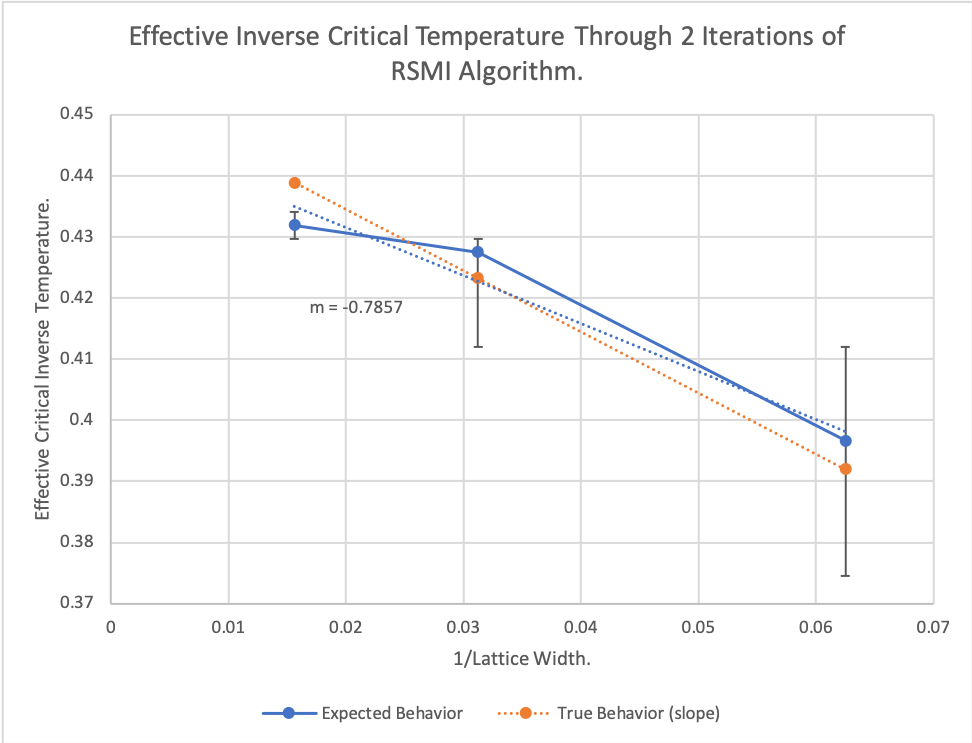
\includegraphics[width=0.75\textwidth]{figures/crit-exponent.png}
  \caption{The finite-size scaling curve for the correlation length
    critical exponent.\label{fig:nu} }
\end{figure}
In fact, this result is just the start. Our investigation revealed a
large number of possible improvements and generalizations. Due to the
time contraints of this capstone, we have not yet implemented these
ideas, but, all the same, these ideas merit attention. The
generalization we discuss gives rise to a family of RSMI-inspired
techniques, together constituting a new branch of RG methods.

\section{A Generalization to $n$-Spin and $O(n)$ Systems}
Koch-Janusz and Ringel claim the RSMI algorithm works for general
lattice systems.  However, the current formulation works only for
systems with binary degrees of freedom: spin-$1/2$ Ising models. The
authors avoid explicitly generalizing these results.  Though the
generalization is straightforward, it is important enough to warrant
elaboration.

Let us consider systems with either $n$ spins or $n$ components of spin, then, the visible
units of our RBM should be able to take $n$ values. Accomplishing this
is quite simple: we let our visible units become vectors with $n$
components: $v_i\rightarrow \{v_{id}\}_{d=1}^n$.  We say that $v_i$
takes the value of spin $d$ when:
\begin{equation}%
  v_i \equiv d \iff
  \begin{cases}
    v_{id}=1\\
    v_{id'}=0, d'\neq d.
  \end{cases}
\end{equation}%
In fact, we will use the RBM to model a slightly different vector:
\begin{equation}%
  v_{id}=P(d),
\end{equation}%
where the vector is normalized $\sum_d v_{id}=1$. Such a vector that contains
probabilities of classes is called a \textit{one-hot
encoding}, and with these probabilities, we can randomly sample values
of spin to generate $n$-valued spins. For $n$-vector models, we leave
the probabilities as they are. To allow our RBMs to produce these
encoding, we have to introduce the index $d$ in the parameters of our
model:
\begin{align}%
  a_i &\rightarrow a_{id}\\
  w_{ij}&\rightarrow w_{ijd}.
\end{align}%
To derive a one-hot encoding, we change the RBM's reverse update rule,
$P(\bv\rvert \bh)$ (\ref{eq:h-to-v}).  The conditional probabilities
will still factor, but normalization over the scalar values $v_i=0,1$,
becomes normalization over the components of the vector, $d$.  If we
denote $\epsilon_i \eqcolon -(\sum_j w_{ij} h_j + a_i )$, then, whereas
before, we had:%
\begin{equation}%
  P(v_i\rvert\bh)=\frac{e^{-\epsilon_i v_i}}{\sum_{v_i'\in\{0,1\}} e^{-\epsilon_i v_i'}},
\end{equation}%
now we have, $\epsilon_{id}\eqcolon-(\sum_j w_{ijd}h_j+ a_{id})$, so:
\begin{equation}%
  P(v_{id}\rvert\bh)=\frac{e^{-\epsilon_{id} v_{id}}}{\sum_{d=1}^n e^{-\epsilon_{id} v_{id}'}}.
\end{equation}%
For $n=2$, we rederive the previous rule with a suitable choice in
$w_{id}$, $a_{id}$. For reasonable values of $d$ (anything we might
encounter in practice), we can perform these calculations
explicitly. If we apply this change to each of the RBMs in the RSMI
algorithm, we will be able to model $n$-spin and $O(n)$
models. Note that since we did nothing to the hidden variables, these
will still be either binary or Bernoulli-valued. If we require that
the hidden spins take the same form as the input variables, as we
might demand with RG, then we also need to apply a completely
analogous change to the hidden unit of the $P(h_j\rvert \bv^{(j)})$
RBM, and we can apply the RSMI algorithm to generic lattice systems.

There is, in fact, more room for generalization. Consider an arbitrary
Hamiltonian for a system with binary-valued data $H(\bx)$. If we
Taylor expand this function, we would get:%
\begin{equation}%
  H(\bx)= a + \sum_i b_i x_i + \sum_{ij}c_{ij} x_i x_j.
\end{equation}%
These are \textit{all} the terms in the expansion.\footnote{For $p>1$,
  $x_i^p = 0$ or $1$.}  Then, barring the bipartite structure, the RBM
energy function already has the most general form we could possibly
consider.  However, when we make the switch to continuous or $n$-ary
valued data, this is no longer true: the Taylor-expansions become
infinite. In these cases, we might consider energy functions with
different, possibly higher-order interactions.  As long as we maintain
the bipartite structure, we can ensured that conditional probabilities
factor. Then, we can use variants of contrastive-divergence to
efficiently train these models. We need not even require that
$P(\bv\rvert\bh)$ and $P(\bh\rvert\bv)$ take the same form.  The first
might be Gaussian and the second a gamma distribution. Formally, we
can consider the extension of RBMs into the \textit{exponential
  family}, and for a full discussion of the possibilities, we refer
the reader to~\cite{welling}.  Suffice to say, there are more powerful
options for modeling probability distributions. Though the current
choices suffice for the spin-$1/2$ Ising model, these extensions may
prove necessary in investigating more complicated systems.

For all the exact results of Koch-Janusz and Ringel, their practical
implementation uses a proxy which does not fully capture the above
mutual information~\cite{kjr}. Here we see two possibilities. First, we can
improve Koch-Janusz and Ringel's approximation. The authors use a
cumulant expansion
\begin{equation}%
  \expect{\exp\{K(\bx)\}}=e^{\sum_{\k=0}^\infty\frac{1}{\k!} C_{\k}},
\end{equation}%
with cumulants expressed in terms of the moments
\begin{align}%
  C_1&=\expect{K},\\
  C_2&=\expect{K^2}-\expect{K}^2,\\
  C_3&=\expect{K^3}-3\expect{K^2}\expect{K}+2\expect{K}^3,\\
\end{align}%
and so on. In deriving the proxy, only the first term is kept
\sref{sec:rsmi-calc}. For better results, a first improvement could be
made by introducing additional terms.\footnote{We may even be able to
  avoid this expansion altogether, see \fref{sec:rsmi-calc}.} Second,
we can consider other approximations of the mutual information, and we
draw the reader's attention to a sampling of options in the
literature: contrastive predictive coding~\cite{oord}, Deep
InfoMax~\cite{hjelm}, and Mutual Information Neural
Estimation~\cite{belghazi}. All three examples use mutual information
as the basis for powerful unsupervised techniques. Though we avoid
details, similarities (and differences) with the RSMI algorithm
warrant further investigation.

Perhaps the most exciting future course of action is extending these
ideas to momentum-space renormalization. Rather than focus on lattice
models, our goal would be to solve quantum field theories. A first
attempt might use the quantum-to-classical mapping of the path
integral formalism~\cite{kjr}. More powerful however would be to use
the same physical and information-theoretic arguments to devise
conditions equivalent to \fref{eq:rsmi} from first fundamentals.
